Para el desarrollo de este proyecto, se hizo un estudio de mercado tanto de los
consumidores como de sus características, además de una evaluación exhaustiva
de qué les gustaría tener en su vehículo.

Este proyecto pretende en un futuro salir a mercado y suplir características que los
usuarios echan en falta en sus correspondientes medios de transporte. Como en principio
funciona con cualquier vehículo que cuente con \ac{OBD}--II, las respuestas no se han
limitado a aquellos conductores que tuviesen turismos sino cualquier tipo de
automóvil: motocicleta, camión, etc.

Es importante destacar que el estudio tiene varios sesgos que han restringido
y delimitado las respuestas que se han registrado, a saber:

\begin{enumerate}
  \item Se ha realizado un cuestionario usando Google Forms, una plataforma de Google
        que permite preparar una serie de preguntas y respuestas y aplicar ciertos
        filtros sobre ellas. Por ejemplo, para aquellos que dijeron ser conductores,
        se hicieron preguntas diferentes frente a quienes no lo fueran.

        Esto permite obtener datos más fidedignos y acotados según la población que
        respondiera. Sin embargo, tiene una limitación implícita: restringe el acceso
        a aquellos con conocimientos ``suficientes'' acerca de la plataforma. Pese
        a que el producto de Google pretende ser lo más accesible posible, no hay
        que olvidar que este tipo de tecnologías permanecen desconocidas para una
        gran parte de la población con escasos conocimientos acerca de Internet o
        del mundo informático. Se comentará más adelante, pero esto se ve reflejado
        principalmente en la edad media de quienes respondieron el cuestionario.

        Por otra parte, al ser un cuestionario aparece otra limitación implícita
        que es la validación y verificación de las respuestas: se confía en la buena
        fe de los participantes y en la calidad de sus respuestas. Igualmente, se
        desarrolló el cuestionario junto con una psicóloga que ayudó a definir
        preguntas cerradas e incluir algunas que sirvieron de control. Por otra parte,
        se usó el propio mecanismo que ofrece este servicio de Google para ordenar
        aleatoriamente las respuestas del cuestionario (y que eso sirviese también
        como control).

  \item Los encuestados fueron contactados principalmente por la red social Twitter,
        mediante la difusión con ``me gusta'' y ``\textit{retweet}''. También se usaron otros
        medios de comunicación (como el correo UPM y Telegram/WhatsApp), pero el
        mayoritario fue el ya mencionado. Nuevamente, esto introduce un sesgo tanto
        por edad como por accesibilidad, ya que pese a ser una red social ampliamente
        utilizada limita el acceso a aquellos que la usen con relativa frecuencia.

  \item Junto con la encuesta, se realizó un sorteo entre aquellos que respondiesen
        a la misma de un cheque regalo de Amazon valorado en 20\EUR{}. Si bien este
        incentivo pudiera resultar interesante, puede resultar también en un nuevo
        sesgo en donde personas que o bien no compren en Amazon o bien no sepan
        lo que es no quisieran hacer el cuestionario.

        Además, se plantea la casuística en que ciertas personas quisieran responder
        al cuestionario solo por el cheque de Amazon, sin importar la calidad de
        las respuestas, ``ensuciando'' los resultados obtenidos y quitándole credibilidad
        al cuestionario en sí.

        Esto se analizará posteriormente junto con las respuestas recibidas y las
        preguntas de control introducidas.

  \item El cuestionario, al ser relativamente exhaustivo, pudo echar para atrás a muchos
        posibles encuestados ya que se estima que el tiempo medio para realizarlo es del
        orden de 10/15 minutos. A parte del daño evidente de tener menos muestra con la
        que trabajar, este posible suceso reduciría también la variedad de la población
        y la calidad del estudio realizado.
\end{enumerate}

Sin más demora, se van a analizar las distintas respuestas.

La primera pregunta que se realizó a los encuestados era si eran conductores o no.
Los datos revelan que el $72.7\%$ ($16$) de los encuestados son conductores, mientras que el
$27.3\%$ ($6$) restantes no, del total que fueron $22$ (figura \ref{fig:drivers-nodrivers}):

\begin{figure}[H]
  \centering
  \includegraphics[width=\linewidth]{images/drivers-nodrivers.png}
  \caption{Proporción de conductores (en azul) frente a no conductores (en rojo) sobre el total de encuestas realizadas.}
  \label{fig:drivers-nodrivers}
\end{figure}

Sobre aquellos que dijeron ser conductores, se preguntó acerca de los años que
llevaban con carnet de conducir, así como los tipos de carnet de conducir que tenían
los encuestados.

Se vio que un $68.8\%$ tenía el carnet desde hace 3 años o más ($11$ encuestados
en particular); un $12.5\%$ tenía el carnet desde hace solo un año ($2$ encuestados)
y el restante, en su mayoría, tenía el carnet desde hace menos de un año. Esto se ve
reflejado en el histograma \ref{fig:carnet-time-hist}:

\begin{figure}[H]
  \centering
  \includegraphics[width=\linewidth]{images/carnet-time.png}
  \caption{Histograma que muestra los años de carnet de los encuestados.}
  \label{fig:carnet-time-hist}
\end{figure}

Con respecto a los tipos de carnet, el $100\%$ de los encuestados (que dijeron ser
conductores) tiene el carnet tipo B. Se vio que el $18.8\%$ tiene además los
carnets relativos a las motocicletas (muy posiblemente, los encuestados tienen el
carnet tipo ``A'' que les habilita automáticamente para aquellos de menor nivel,
como el AM, A1 y A2); y únicamente un encuestado tiene el carnet tipo C, que permite
conducir camiones.

Una restricción que se comentó con anterioridad era la edad media de los participantes.
Esta pregunta se realizó por dos motivos:

\begin{enumerate}
  \item Definir estadísticamente la edad media de la población para una posterior evaluación
        de su longevidad y experiencia tanto en la conducción como en la posible
        compra-venta de vehículos.
  \item Diferenciar, definir y clasificar los encuestados por grupos de edad y descubrir
        posibles sesgos y restricciones en las respuestas para un posterior análisis
        sobre la causa de dichos sesgos y restricciones.
\end{enumerate}

Es necesario decir que solo se preguntó por la edad a aquellas personas que respondieron
afirmativamente a ser conductores. Esto se hizo así debido a que sus respuestas han
conformado el dato más relevante a la hora de realizar la investigación, y se hace así
también estadísticamente.

Se tiene pues que:

\begin{equation}\label{eq:ages}
  \left\{\begin{aligned}
    X_{min}               & = 19               \\
    \bar{X}               & = 30               \\
    Mediana\left(X\right) & = 26.5             \\
    S\left(X\right)       & \approx \pm 10.564 \\
    X_{max}               & = 55
  \end{aligned}\right.
\end{equation}

Se presenta a continuación (figura \ref{fig:ages}) la proporción de edades de los
encuestados frente al total de encuestas realizadas.

\begin{figure}[H]
  \centering
  \includegraphics[width=\linewidth]{images/ages-pie.png}
  \caption{Distribución de edades de los encuestados (valor previo al paréntesis) y su proporción frente al total.}
  \label{fig:ages}
\end{figure}

Como se puede ver en la ecuación \ref{eq:ages}, la distancia entre los valores
mínimo y máximo es de $36$ puntos. Sin embargo, los valores de la media $\left(\bar{X}\right)$
y la mediana $\left(Mediana\left(X\right)\right)$ muestran que la distribución está
bastante centrada en torno a la media, con una desviación estándar $\left(S\left(X\right)\right)$
de $\approx\pm10.564$.

Es interesante notar los tres grandes bloques presentes en la figura \ref{fig:ages}
que evidencian lo que se venía indicando anteriormente: en proporción, a la encuesta
ha accedido más población joven que adulta. Mismamente, solo el porcentaje de personas
encuestadas con edad por debajo de los 26 años es del $49.9\%$, casi la mitad de
los encuestados. Ampliando dicho margen hasta los 36 años, el porcentaje crece hasta
el $81 \%$.

Este dato se puede ver también reflejado en la distribución de los cuartiles, en donde
se tiene que:

\begin{equation}\label{eq:age-quartiles}
  \left\{
  \begin{aligned}
    Q_1 & = 22.75 \\
    Q_3 & = 33.00
  \end{aligned}
  \right.
\end{equation}

Como se puede apreciar en la ecuación \ref{eq:age-quartiles}, la distribución de
cuartiles está en un rango de edad por debajo de los 33 años para el $75\%$ de la
muestra, indicativo nuevamente de una población encuestada joven.

Destacan dos datos sobre los demás en donde los encuestados tienen 51 y 55 años
respectivamente. De este caso en particular se hablará posteriormente, pero cabe
destacar que sus respuestas fueron las más pobres en cuanto a contenido (sobre todo
en aquellas que sirvieron de control), seguramente debido al formato del
cuestionario, fatiga tras responder las secciones anteriores, etc.

Una vez se indagó acerca de la información que identifica a la muestra, se preguntó
directamente por el vehículo con el que contaban así como las características del
mismo. Para esta sección, se han dividido las preguntas en tres categorías:
\textit{básico}, \textit{habitual} y \textit{premium}. Dichas categorías se crean
según el porcentaje de presencia habitual mundial de las características que se
enumeran en la tabla \ref{tab:car-specs}:

\begin{table}[H]
  \centering
  \begin{tabular}{|c|c|c|}
    \hline
    \textbf{Básico}          & \textbf{Habitual}            & \textit{\textbf{Premium}} \\
    \hline\hline
    Control de crucero       & Pantalla táctil              & Asistente virtual         \\
    Limitador de velocidad   & GPS                          & Aplicación móvil          \\
    Cámara de visión trasera & Detección de ángulos muertos & Cámara \textit{on-board}  \\
    Botón de arranque        & Android Auto                 &                           \\
    \hline
  \end{tabular}
  \caption{Tabla de distribución de las características de los vehículos, preguntado en el cuestionario.}
  \label{tab:car-specs}
\end{table}

Tras el cuestionario, las frecuencias obtenidas fueron:

\begin{figure}[H]

  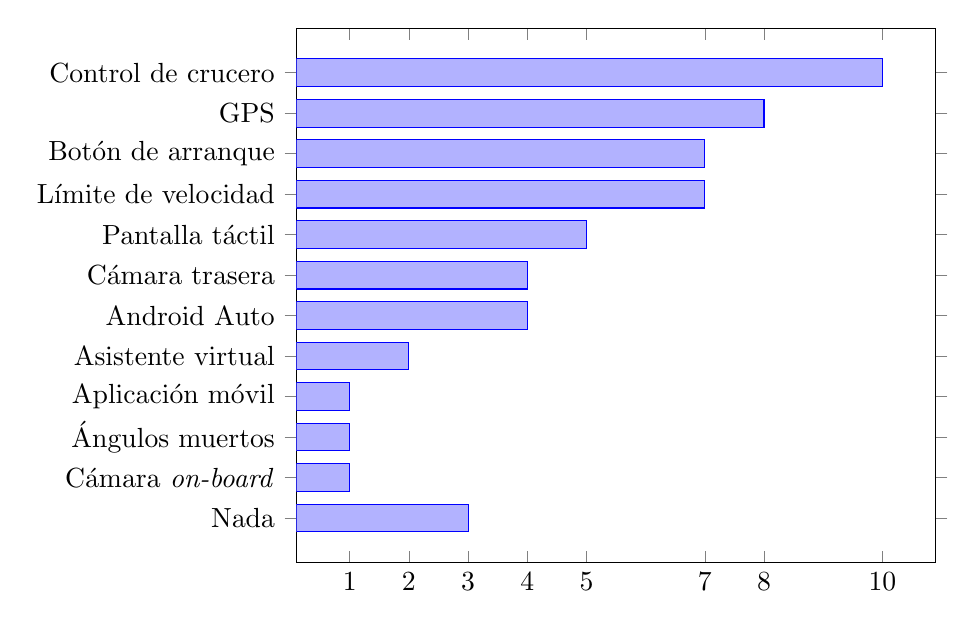
\begin{tikzpicture}
    \begin{axis} [%
        xbar,
        width=.8\linewidth,
        ytick=data,
        yticklabels={%
            Nada,
            Cámara \textit{on-board},
            Ángulos muertos,
            Aplicación móvil,
            Asistente virtual,
            Android Auto,
            Cámara trasera,
            Pantalla táctil,
            Límite de velocidad,
            Botón de arranque,
            GPS,
            Control de crucero,
          },
        xtick=data,
      ]
      \addplot coordinates {
          (3, 0)
          (1, 1)
          (1, 2)
          (1, 3)
          (2, 4)
          (4, 5)
          (4, 6)
          (5, 7)
          (7, 8)
          (7, 9)
          (8, 10)
          (10, 11)
        };
    \end{axis}
  \end{tikzpicture}
  \caption{Distribución de las características de los vehículos de los encuestados.}
  \label{fig:vehicle-specs}
\end{figure}

Como se puede observar en la imagen \ref{fig:vehicle-specs}, una gran mayoría de vehículos
tienen lo que se consideran ``características básicas'', según la tabla \ref{tab:car-specs}.

Es interesante destacar que cada vez más vehículos dentro del parque español cuenta con
diversos elementos de seguridad y confort, como pantalla táctil y navegador \ac{GPS},
incluso por encima de ciertas características básicas. Si bien esto es positivo para
el sector, puede suponer un problema a la hora de sacar a la venta este proyecto ya
que estaría, según los datos recogidos anteriormente, mayoritariamente orientado
a vehículos ``antiguos'' o no tan modernos.

Es por ello por lo que se realizó también una encuesta sorbe edad aproximada de
los vehículos. De la muestra total de 16 conductores, se obtuvieron los siguientes
datos sobre la edad del parque de vehículos encuestados (ecuación \ref{eq:vehicle-age}):

\begin{equation}\label{eq:vehicle-age}
  \left\{
  \begin{aligned}
    X_{min}               & = 2               \\
    \bar{X}               & = 10.12           \\
    Mediana\left(X\right) & = 10.00           \\
    S\left(X\right)       & \approx \pm 6.839 \\
    X_{max}               & = 21
  \end{aligned}
  \right.
\end{equation}

En este caso, es muy interesante ver la variedad en las respuestas: entre el mínimo
y el máximo hay casi 20 años; sin embargo, la media y la mediana son casi las mismas,
centradas en torno a los 10 años, con una desviación estándar de aproximadamente
$\pm 6.839$ años.

Para esta estadística es fundamental observar los cuartiles, ya que van a reflejar
datos muy interesantes que darán ciertas pistas sobre las especificaciones de los
vehículos, que se habló anteriormente en la figura \ref{fig:vehicle-specs}:

\begin{equation}\label{eq:vehicle-age-quartiles}
  \left\{
  \begin{aligned}
    Q_1 & = 3.5  \\
    Q_3 & = 14.5
  \end{aligned}
  \right.
\end{equation}

Como se puede observar en los cuartiles \ref{eq:vehicle-age-quartiles}, el $25\%$ de
la muestra se localiza en los primeros $\left[0, 3'5\right]$ años de antigüedad, y el
$75\%$ de la muestra es abarcada para todos los vehículos de hasta $14.5$ años de
antigüedad.

Esta información es muy relevante ya que gran parte de la muestra se corresponde con
vehículos bastante nuevos, y eso explica en parte el porqué de los resultados obtenidos
en la encuesta acerca de las características, representada por la figura \ref{fig:vehicle-specs}.
Cabe destacar que la moda de la distribución es:

\begin{equation}\label{eq:vehicle-age-mode}
  M\left(X\right) = 2
\end{equation}

con 4 de los 16 encuestados teniendo un vehículo de 2 años de edad, lo que se traduce
en un parque muy moderno. Sin embargo, esto también ha servido para desvelar nuevas
necesidades que no existían antes y que los nuevos vehículos no son capaces de
suplir.

Con la encuesta ``personal'' ya completada, se dio paso en el cuestionario a una
evaluación de características que \ac{VIMS} debería incluir. La primera pregunta era
un listado de 20 características que pueden ser medidas mediante el \ac{OBD}--II
y un sistema de puntuaciones escalado del 1 al 20. Cuanto más pequeño fuese el valor,
más importante se considera que es esa característica para el encuestado. Las preguntas
realizadas se muestran en la tabla \ref{tab:quest-options}:

\begin{table}[H]
  \centering
  \begin{tabularx}{\textwidth}{| C{.25} | C{.25} | C{.25}| C{.25} |}
    \hline
    Visualización en tiempo real   & Información detallada de errores & Velocímetro                  & Cuentarrevoluciones                        \\
    \hline
    Marcha actual (1ª, 2ª, \dots)  & Temperatura del aceite           & Presión del aceite           & Temperatura exterior                       \\
    \hline
    Intensidad del acelerador (\%) & Consumo actual                   & Presión de las ruedas        & Presión de los inyectores                  \\
    \hline
    Nivel de combustible           & Distancia recorrida              & Nivel de batería             & Nivel de carga en valor absoluto del motor \\
    \hline
    Presión atmosférica            & Temperatura de la toma de aire   & Temperatura del refrigerante & Temperatura del motor                      \\
    \hline
  \end{tabularx}
  \caption{Opciones ofrecidas a los encuestados. Se han escogido diversas opciones que se encuentran entre los datos habituales generados por un vehículo.}
  \label{tab:quest-options}
\end{table}

Es importante destacar que la tabla anterior contiene valores puramente técnicos,
en donde solo aquellos con un conocimiento más específico entenderán y sabrán
interpretar; y otros más genéricos que en principio todos los conductores conocen
(como velocidad actual, temperatura del aceite del motor, \dots).

Las respuestas a las preguntas anteriores se han estructurado en dos tablas: una
primera que representa toda la población en general, y una segunda en donde solo
están las respuestas de los conductores (tabla \ref{tab:answer-population} y tabla
\ref{tab:answer-drivers}):

\begin{table}[H]
  \centering
  \begin{minipage}{.48\linewidth}
    \begin{tabularx}{\textwidth}{|C{.3}|C{.7}|}
      \hline
      \textbf{Puntuación} & \textbf{Opción}                            \\
      \hline
      1                   & Velocímetro                                \\
      1                   & Nivel de combustible                       \\
      4                   & Marcha actual                              \\
      5                   & Distancia recorrida                        \\
      5                   & Nivel de batería                           \\
      6                   & Cuentarrevoluciones                        \\
      8                   & Intensidad del acelerador (\%)             \\
      8                   & Presión de las ruedas                      \\
      10                  & Temperatura del aceite                     \\
      10                  & Nivel de carga en valor absoluto del motor \\
      12                  & Visionado en tiempo real                   \\
      12                  & Consumo actual                             \\
      12                  & Temperatura del motor                      \\
      14                  & Presión del aceite                         \\
      14                  & Temperatura del refrigerante               \\
      16                  & Presión atmosférica                        \\
      17                  & Temperatura exterior                       \\
      19                  & Información detallada de errores           \\
      19                  & Presión de los inyectores                  \\
      20                  & Temperatura de la toma de aire             \\
      \hline
    \end{tabularx}
    \caption{Puntuaciones obtenidas de forma general, por la población al completo (conductores y no conductores).}
    \label{tab:answer-population}
  \end{minipage}
  \hfill
  \begin{minipage}{.48\linewidth}
    \begin{tabularx}{\textwidth}{|C{.3}|C{.7}|}
      \hline
      \textbf{Puntuación} & \textbf{Opción}                   \\
      \hline
      1                   & Velocímetro                       \\
      1                   & Nivel de combustible              \\
      3                   & Temperatura del motor             \\
      4                   & Temperatura del aceite            \\
      4                   & Nivel de batería                  \\
      5                   & Distancia recorrida               \\
      6                   & Cuentarrevoluciones               \\
      7                   & Presión de los inyectores         \\
      8                   & Presión de las ruedas             \\
      10                  & Presión del aceite                \\
      11                  & Marcha actual                     \\
      11                  & Presión atmosférica               \\
      14                  & Temperatura del refrigerante      \\
      15                  & Temperatura exterior              \\
      17                  & Intensidad del acelerador (\%)    \\
      18                  & Información detallada de errores  \\
      18                  & Consumo actual                    \\
      19                  & Temperatura de la toma de aire    \\
      20                  & Visionado en tiempo real          \\
      20                  & Nivel de carga absoluta del motor \\
      \hline
    \end{tabularx}
    \caption{Puntuaciones obtenidas de forma general, por la población (excluidos los no conductores).}
    \label{tab:answer-drivers}
  \end{minipage}
\end{table}

De los datos anteriores es interesante ver cómo ciertos campos cambian completamente
de ubicación según ha respondido la población general o solo los conductores, como por
ejemplo la temperatura del motor. Otras, por el contrario, es interesante que se mantengan
en la misma posición según las tablas, como el velocímetro. Este caso en particular
resulta especialmente interesante ya que es un elemento que tienen todos los vehículos.
Sin embargo, tanto la población en general como la comunidad de conductores lo ha
puntuado como el elemento de más interés sobre el que obtener datos.

De las características puntuadas en las tablas \ref{tab:answer-population} y \ref{tab:answer-drivers}
se extraerán una serie de componentes que se detallan en mayor profundidad en el
punto \ref{ssec:user-req}, la obtención de los requisitos de usuario.

A continuación, se realizaron una serie de preguntas de desarrollo, en donde el
encuestado tenía libertad para poder exponer ideas y opiniones sobre ciertas
características del coche. Esta sección sirvió en parte como sección de control
y también ha permitido definir con mayor certeza ciertas restricciones del cuestionario,
como su accesibilidad. También ha permitido descubrir el porqué de ciertas puntuaciones
especialmente elevadas.

La primera pregunta que se realizó fue: ``\textbf{?`Qué te gustaría poder medir de tu coche?}'',
de la cual se extrajeron ciertas ideas interesantes:

\begin{itemize}
  \item El velocímetro en digital, que explica el porqué tiene una puntuación tan alta.
  \item Información relativa al estado del coche: nivel de aceite, presión de las ruedas, líquido de frenos, \dots
  \item Nivel de gasto de combustible con respecto al histórico de otros meses.
  \item Consumo de combustible actual y estimación de kilómetros.
  \item Información referente al estado mecánico del vehículo que pueda ayudar a prevenir averías.
  \item Ubicación de aparcamiento.
  \item Vida útil de la batería del motor eléctrico.
  \item Recorrido seguido durante un trayecto.
\end{itemize}

Como se puede apreciar, gran parte de las respuestas van orientadas a prevenir fallos
mecánicos, a estimaciones de combustible y generación de información de los viajes
(la enumeración anterior es un resumen de las respuestas totales -- hay repeticiones
entre ellas). Es interesante que ciertas respuestas ya se habían contemplado en
la primera etapa de diseño del proyecto, y reafirman lo que se busca desde el
comienzo: que el usuario recupere el control sobre su vehículo.

A continuación, se realiza una segunda pregunta muy parecida a la primera que se usó
como control (\textbf{?`Qué información echas en falta en tu uso habitual del coche?}).
Esta pregunta se ha ignorado ya que se utilizó principalmente para verificar la
coherencia entre las respuestas. Algunos usuarios aportaron algunas ideas nuevas
de elementos que querrían medir, otros copiaron la respuesta anterior (que se
consideró válido dada la índole de la pregunta) y otros hicieron referencia a
características ya descritas en la pregunta anterior.

Otra pregunta que se hizo fue ``\textbf{Si tuvieras que añadirle una característica al
coche, ?`cuál sería?}'', en donde el usuario se podía poner ``imaginativo'' y comentar
qué querría que tuviese su vehículo. De las respuestas, las hubieron muy variadas
y distintas, y solo se muestran aquí algunas que podrían ser implementadas con
\ac{VIMS}:

\begin{itemize}
  \item Presión de las ruedas.
  \item Aviso de errores.
  \item Desgaste de las ruedas.
  \item Calidad del aire del habitáculo.
  \item Emisiones de $CO_2$ y advertencia ante fuertes temperaturas.
\end{itemize}

Finalmente, se preguntó por ciertas acciones que resultarían de interés el
automatizarlas, también sin restricción en las respuestas. Algunas respuestas
fueron:

\begin{itemize}
  \item Reset del odómetro.
  \item Aviso de mantenimientos recomendados según kilometraje -- ruedas, aceite, frenos, etc.
  \item Generación de estadísticas del viaje para trayectos de más de 30 minutos según
        las características mencionadas en las preguntas anteriores.
\end{itemize}

Estas respuestas fueron muy útiles para generar y definir los requisitos de usuario:
a fin de cuentas, el usuario es el \textit{stakeholder} principal y satisfacer sus
necesidades debe ser la principal prioridad (y desde aquí, muchas gracias a todos
ellos por responder). La selección final de los datos que serán leídos
por \ac{VIMS} se detalla en el punto \ref{ssec:user-req}.

Como se ha mencionado anteriormente, el cuestionario presenta de partida ciertas
restricciones para aquellos que quieran participar. Por una parte, al ser un cuestionario
puramente \textit{online}, el acceso ya está restringido de base a aquellos con
conocimiento suficiente o un uso hábil de la tecnología (esto se ha podido ver
en la ecuación \ref{eq:ages} y en la imagen \ref{fig:ages} con respecto a la medición
de la edad). Por otro lado, otra restricción existente es el conocimiento de los
participantes con respecto al tema que se preguntaba.

Para evaluar las restricciones, se introdujo una última pregunta en la que se
solicitaba a los encuestados añadir alguna sugerencia o comentario que tuviesen con
respecto al cuestionario. Además, se evaluó el lenguaje utilizado para responder las
preguntas y se realizó un análisis sobre dichas respuestas.

Por una parte, se indicó que responder y puntuar las características no resultó
cómodo, sobre todo en dispositivos móviles donde la pantalla es mucho más pequeña.
Se usó el formato matricial ofrecido por Google Forms, pero el problema surgió
por el tamaño de la matriz, $20 \times 20$, excesivamente grande en según qué
dispositivo se respondiese al cuestionario.

Otra sugerencia que se repitió con más o menos frecuencia fue la de la accesibilidad
y fluidez del producto final. Un encuestado con un vehículo relativamente nuevo
mencionaba lo molesto que le resulta interactuar con la pantalla de su vehículo y notar
retardo en las acciones, que se quedase bloqueado abriendo aplicaciones, etc., lo cual
le transmitía la sensación de que contaba con un vehículo antiguo y de mala calidad.
Esto se produce, entre otros factores, porque no se desarrollan labores de optimización
en los dispositivos integrados de los vehículos, en este caso, la pantalla.

Siguiendo la misma línea, otro usuario mencionaba que querría que el producto final
fuese simple y fácil de entender a primera vista, evitando el exceso de datos y la
complejidad de la interfaz de usuario final.

Por otro lado, finalizando con lo que se planteó al inicio de este apartado, se
estudió la ``calidad'' de las respuestas, en especial en los sujetos cuya edad
era bastante superior a la media. Es notorio que dichos sujetos, en las preguntas
de desarrollo, indicasen en todas las ocasiones ``\textit{Ns/nc}'' (\textit{No Sabe/No Contesta}).
Tras evaluarlo con cierto detenimiento (teniendo en cuenta la buena fe de los
participantes y sabiendo personalmente quiénes son), se deduce que el cuestionario resultó
excesivamente largo y complejo para el sector
más longevo de la población. Esto pudo dificultar el responder al mismo debido
a la fatiga, el tiempo que llevaba o lo técnico que pudiera resultar el lenguaje,
afectando directamente a la calidad de las respuestas.

Se vio cómo además ciertos usuarios tuvieron dificultad al responder al cuestionario
debido a los tecnicismos o palabras propias del sector que pudieran usarse. Un
ejemplo es la palabra ``odómetro'' (también conocido como cuentakilómetros, aunque
nunca se uso ese sinónimo ni se mencionó), que resultó ser desconocida para varios encuestados.

Estas restricciones se comentarán más adelante, en el punto \ref{chap:conclussions},
sobre cómo abordarlas si se volviese a repetir el estudio, junto con ciertas mejoras
en el planteamiento del cuestionario.
